\documentclass{beamer}
%Для защит онлайн лучше использовать разрешение 16x9
%\documentclass[aspectratio=169]{beamer}

%%% Обязательные пакеты
%% Beamer
\usepackage{listings}

\usepackage{beamerthemesplit}
\usetheme{SPbGU}
\beamertemplatenavigationsymbolsempty
\usepackage{appendixnumberbeamer}

%% Локализация
\usepackage{fontspec}
\setmainfont{CMU Serif}
\setsansfont{CMU Sans Serif}
\setmonofont{CMU Typewriter Text}
%\setmonofont{Fira Code}[Contextuals=Alternate,Scale=0.9]
%\setmonofont{Inconsolata}
% \newfontfamily\cyrillicfont{CMU Serif}

\usepackage{polyglossia}
\setdefaultlanguage{russian}
\setotherlanguage{english}
\usepackage[autostyle]{csquotes} % Правильные кавычки в зависимости от языка

%% Графика
\usepackage{wrapfig} % Позволяет вставлять графику, обтекаемую текстом
\usepackage{pdfpages} % Позволяет вставлять многостраничные pdf документы в текст

%% Математика
\usepackage{amsmath, amsfonts, amssymb, amsthm, mathtools} % "Адекватная" работа с математикой в LaTeX

% Математические окружения с русским названием
\newtheorem{rutheorem}{Теорема}
\newtheorem{ruproof}{Доказательство}
\newtheorem{rudefinition}{Определение}
\newtheorem{rulemma}{Лемма}

%%% Дополнительные пакеты. Используются в презентации, но могут быть отключены при необходимости
\usepackage{tikz} % Мощный пакет для создание рисунков, однако может очень сильно замедлять компиляцию
\usetikzlibrary{decorations.pathreplacing,calc,shapes,positioning,tikzmark}

\usepackage{multirow} % Ячейка занимающая несколько строк в таблице

%% Пакеты для оформления алгоритмов на псевдокоде
\usepackage[noend]{algpseudocode}
\usepackage{algorithm}
\usepackage{algorithmicx}

\usepackage{fancyvrb}


% То, что в квадратных скобках, отображается внизу по центру каждого слайда.
\title[RISC-V Instrew]{Динамическая бинарная трансляция в RISC-V с помощью Instrew}

% То, что в квадратных скобках, отображается в левом нижнем углу.
\institute[СПбГУ]{}

% То, что в квадратных скобках, отображается в левом нижнем углу.
\author[Михайлов Илья]{Михайлов Илья Игоревич, группа 21.Б07-мм}

\begin{document}
{
\setbeamertemplate{footline}{}
% Лого университета или организации, отображается в шапке титульного листа
\begin{frame}
  \includegraphics[width=1.4cm]{pictures/SPbGU_Logo.png}
  \vspace{-35pt}
  \hspace{-10pt}
  \begin{center}
    \begin{tabular}{c}
      \scriptsize{Санкт-Петербургский государственный университет} \\
      \scriptsize{Кафедра системного программирования}
    \end{tabular}
    \titlepage
  \end{center}

  \btVFill

  {\scriptsize
    % У научного руководителя должна быть указана научная степень
    \textbf{Научный руководитель:} Д.С. Косарев, ассистент кафедры системного программирования \\
    % Консультанта может и не быть. Должна быть указана должность или ученая степень
    % \textbf{Консультант:}  П.П. Петров, программист ЗАО \enquote{Компания с ну очень-очень-очень длинным названием}\\
    % Для курсовой не обязателен. Должна быть указана должность или ученая степень
    % \textbf{Рецензент:} д.т.н., проф. И.И. Иванов, исполнительный директор ООО \enquote{Рога и копыта}
  }
  \begin{center}
    \vspace{5pt}
    \scriptsize{Санкт-Петербург\\
      2024}
  \end{center}

\end{frame}
}

% \begin{frame}[fragile]
%   \frametitle{Введение}
%   \begin{itemize}
%     \item Краткий обзор тематики работы (как вариант~--- устно, пока показывается титульный слайд)
%     \item Не нужно определять общеизвестные понятия
%     \item Применимость/полезность данной работы, обоснование выбора именно этой темы
%     \item Если тема похожа на темы других работ (в том числе прошлых лет), надо явно описать разницу
%   \end{itemize}
% \end{frame}

\begin{frame}[fragile]
  \frametitle{Введение}
  \begin{itemize}
    \item Бинарные трансляторы являются инструментами для анализа кода, профиляции и эмуляции
    \item Важным классом которых являются динамические бинарные трансляторы (далее --- ДБТ)
    \item В качестве промежуточного представления для ДБТ хорошо использовать LLVM IR
          \begin{itemize}
            \item Тулчейн LLVM позволяет проводить качественные оптимизации
          \end{itemize}
    \item Хотим ДБТ для RISC-V
          % \item Instrew является ДБТ с поднятием двочиного кода в LLVM IR, но нет поддержки RISC-V, как хост архитектуры
          % \item В результате работы хотим добавить поддержку архитектуры RISC-V для ДБТ с открытым исходным кодом
  \end{itemize}
\end{frame}

% \begin{frame}
%   \frametitle{Существующие решения (инструменты, подходы, алгоритмы)}
%   \begin{itemize}
%     \item Перечислить инструменты/подходы, применяемые в области
%     \item Указать их преимущества и недостатки (критика существующих решений/подходов)
%   \end{itemize}

% \end{frame}

\begin{frame}
  \frametitle{Обзор}
  \begin{itemize}
    \item Динамические бинарные трансляторы:
          \begin{itemize}
            \item QEMU-user
            \item Rosetta 2
            \item Valgrind
            \item Box64
          \end{itemize}
    \item Динамические бинарные трансляторы с поднятием в LLVM IR:
          \begin{itemize}
            \item Instrew + Rellume
	    \item BinRec, HQEMU (не обновлялись с 2022 и 2018 года соответственно)
	    \item DBILL, LnQ, Lasagne (есть только статьи, либо код закрыт)
          \end{itemize}
%    \item Выводы:
%          \begin{itemize}
%            \item Благодаря тулчейну LLVM Instrew производительнее, чем QEMU и Valgrind, а так же имеет API для добавления инструментов бинарного анализа "из коробки"\footnote{\href{https://mediatum.ub.tum.de/doc/1614897/1614897.pdf}{https://mediatum.ub.tum.de/doc/1614897/1614897.pdf}}
%            \item Из всех рассмотренных ДБТ с поднятием в LLVM IR Instrew + Rellume поддерживается мейнтейнером и уже имеет guest-поддержку RISC-V
%          \end{itemize}
  \end{itemize}
\end{frame}

\begin{frame}
  \frametitle{Обзор}
  \begin{itemize}
    \item Выводы:
          \begin{itemize}
	      \item Instrew производительнее, чем QEMU и Valgrind (основываясь на бенчмарках\footnote{\href{https://mediatum.ub.tum.de/doc/1614897/1614897.pdf}{https://mediatum.ub.tum.de/doc/1614897/1614897.pdf}})
	    \item Instrew "из коробки" имеет API для добавления инструментов бинарного анализа
	    \item Из всех рассмотренных ДБТ с поднятием в LLVM IR Instrew + Rellume поддерживается мейнтейнером
	    \item Instrew уже имеет guest-поддержку RISC-V
          \end{itemize}
  \end{itemize}
\end{frame}

% \begin{frame}
%   \frametitle{Существующие решения}
%   Возможно, предметная область сложна и потребуется больше одного слайда, но затягивать введение не стоит. Постарайтесь уложиться в 1--2 слайда
%   \begin{itemize}
%     \item Выводы
%           \begin{itemize}
%             \item Подвести итог
%             \item Указать недостатки существующих подходов, на борьбу с которыми
%                   направленна данная работа
%             \item Чётко сформулировать существующую проблему, которая будет решаться в данной работе
%           \end{itemize}
%   \end{itemize}
% \end{frame}


% Обязательный слайд: четкая формулировка цели данной работы и постановка задачи
% Описание выносимых на защиту результатов, процесса или особенностей их достижения и т.д.
% \begin{frame}
%   \frametitle{Постановка задачи}
%   \textbf{Целью} работы является решение какой-то проблемы %озвученной выше

%   \textbf{Задачи}:
%   \begin{itemize}
%     \item Выбрать алгоритм, подход, метод %основываясь на проведённом анализе проблемы, области, существующих решений
%     \item Разработать алгоритм, делающий то-то с тем-то
%     \item Доказать корректность алгоритма
%     \item Реализовать предложенный алгоритм
%     \item Провести экспериментальное исследование предложенной реализации
%   \end{itemize}
% \end{frame}

%Идеально, если есть по одному слайду на каждую поставленную задачу

\begin{frame}
  \frametitle{Постановка задачи}
  \textbf{Цель:} Добавить поддержку host-архитектуры RISC-V для ДБТ Instrew

  \vspace{5mm}
  \textbf{Задачи:}
  \begin{enumerate}
    % \item Выполнить обзор динамических бинарных трансляторов и сравнить их с Instrew
    % \item Спроектировать то-то
    \item Выполнить обзор архитектуры Instrew
    \item Реализовать минимальную функциональность для запуска Instrew
          на RISC-V:
          \begin{itemize}
            % \item Добавить процессорно-специфические патчи в minilibc и другие компоненты
            % \item Реализовать функции, связанные с RISC-V ABI
            \item Скомпилировать, добавив процессорно-специфические патчи и проставив константы
            \item Реализовать функции, связанные с RISC-V ABI
          \end{itemize}
          % \item Протестировать на простых примерах
    \item Протестировать на простых программах
          % (например на SPEC CPU 2017)
  \end{enumerate}
\end{frame}


% \begin{frame}
%   \frametitle{Алгоритм ABC\footnote{Результаты и обоснования выбора пути достижения цели}}
%   За основу решения взят алгоритм ABC
%   \begin{itemize}
%     \item Почему именно он, а не другие
%     \item Ключевые особенности выбранного алгоритма, важные для решения поставленных задач
%   \end{itemize}
% \end{frame}


% \begin{frame}[fragile]
%   \frametitle{Новый алгоритм\footnote{Иллюстративные возможности: таблицы, картинки, код}}
%   % Задается ширина столбцов
%   \begin{tabular}{p{5cm} p{7cm}}
%     % Фрагмент кода
%     \begin{minipage}{3in}
%       \begin{Verbatim}[commandchars=\\\{\}]

%         \textcolor{blue}{string} res = \textcolor{orange}{""};
%         \textcolor{blue}{for}(i = 0; i < l; i++) \{
%         res = \textcolor{orange}{"()"} + res;
%         \}

%       \end{Verbatim}
%     \end{minipage}
%                 &
%     Результат (SPPF):
%     \\
%     Аппроксимация:
%                 &
%     % Картинка. Изображения должны быть векторными. Исключения --- снимки экрана.
%     \multirow{-2}*{\!\includegraphics[width=6.8cm]{pictures/out3.pdf}}
%     \\
%     \includegraphics[width=2.5cm]{pictures/in3.pdf}
%                 &
%     \\
%     Грамматика: &
%     \\
%     \vspace{-20pt}
%     % Можно формулы писать
%     {\begin{align*}
%          start &  &  & \Coloneq &  & s                                              \\
%          s     &  &  & \Coloneq &  & \mbox{\texttt{LBR }} s \mbox{\texttt{ RBR }} s \\
%          s     &  &  & \Coloneq &  & \epsilon
%        \end{align*}}
%                 &
%   \end{tabular}
% \end{frame}

% \begin{frame}[fragile]
%   \frametitle{Доказательство корректности алгоритма}
%   {\tiny Формулировки утверждений. Идеи доказательств проговариваются устно.}
%   \begin{rutheorem}[Пифагора: геометрическая формулировка]
%     В прямоугольном треугольнике площадь квадрата, построенного на гипотенузе, равна сумме площадей квадратов, построенных на катетах.
%   \end{rutheorem}

%   \begin{rutheorem}[Пифагора: алгебраическая формулировка]
%     В прямоугольном треугольнике квадрат длины гипотенузы равен сумме квадратов длин катетов.

%     То есть, если обозначить длину гипотенузы треугольника через $c$, а длины катетов
%     через $a$ и $b$, получим верное равенство: $a^2 + b^2 = c^2$.
%   \end{rutheorem}

%   \begin{rutheorem}[Обратная теорема Пифагора]
%     Для всякой тройки положительных чисел $a$, $b$ и $c$, такой, что $a^2 + b^2 = c^2$, существует прямоугольный треугольник с катетами $a$ и $b$ и гипотенузой $c$.
%   \end{rutheorem}
% \end{frame}

\begin{frame}[fragile]
  \frametitle{Архитектура Instrew}
  % \begin{itemize}
  %   \item В реализации интересны архитектура, библиотеки, инструменты
  %   \item Не надо добавлять на слайд примеры кода
  % \end{itemize}
  \begin{itemize}
    \item Является клиент-серверной
    \item Работа была проведена над клиентом Instrew
  \end{itemize}
  \begin{figure}
    % 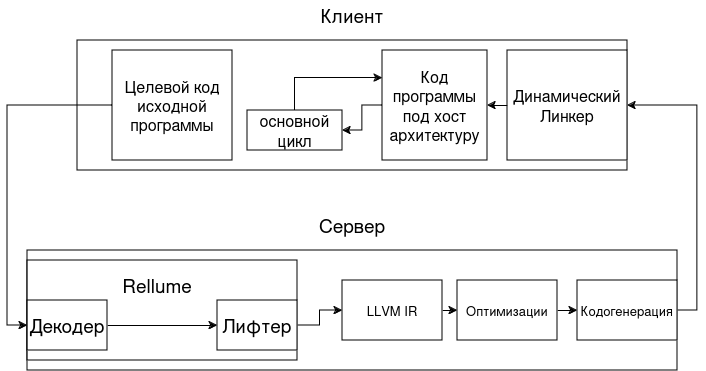
\includegraphics[width=300pt]{pictures/instrew.drawio.png}
    \centering
    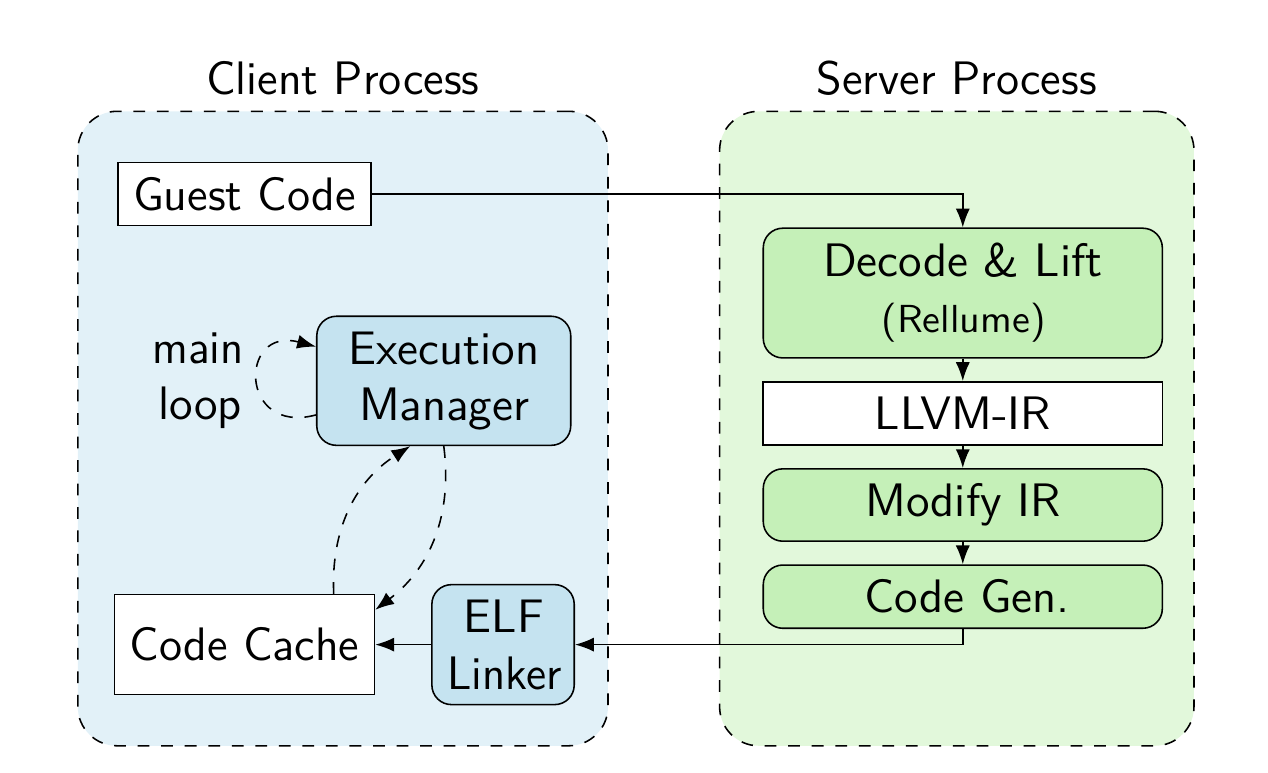
\includegraphics[width=250pt]{pictures/instrew-arch-disser.png}\footnote{диаграмма была взята \href{https://mediatum.ub.tum.de/doc/1614897/1614897.pdf}{отсюда}}
    % \caption{}
  \end{figure}
  % \vspace{-8pt}
\end{frame}

\begin{frame}[fragile]
  \frametitle{Реализация (1/2)}
  \begin{itemize}
    \item Чтобы скомпилировать, необходимо:
          \begin{itemize}
            \item Проставить константы
            \item Написать на ассемблере точку входа в программу
          \end{itemize}
          % \item Из-за недостатка опыта с архитектурой RISC-V, необходимо было прочитать документацию\footnote{https://riscv.org/wp-content/uploads/2017/05/riscv-spec-v2.2.pdf}\footnote{https://github.com/riscv-non-isa/riscv-elf-psabi-doc/blob/master/riscv-elf.adoc}
    \item Оказалось, что не все псевдоинструкции описаны в документации RISC-V\footnote{https://reviews.llvm.org/D49661}
  \end{itemize}
\end{frame}

\begin{frame}[fragile]
  \frametitle{Особенности Instrew (1/2)}
  \begin{itemize}
    \item Клиент Instrew довольно таки непросто диагностировать
    \item Флаги сборки клиента Instrew:
          \begin{itemize}
            % \item -fPIC, -static-pie, -nostdlib, -no-startfiles и т.д.
            % \item В рантайме к instrew-client подключался ld-linux
            % \item Но такого быть не должно, так как instrew-client сам является линкером
            % \item Оказалось, что -static-pie флаг gcc не подразумевал собой -no-dynamic-linker флаг
            \item Клиент во время запуска выдаёт ошибку сегментации
            \item Asan и gprof здесь не работают
%            \item Утилита pmap показывает, что к клиенту динамически линкуется ld-linux и выполнить релокации невозможно
	    \item После локализации ошибки, стало понятно, что к клиенту динамически линкуется ld-linux, чего быть не должно
            \item Оказалось, что --static-pie флаг у gcc-13 на x86\_64 и RISC-V отличается семантикой
          \end{itemize}
    \item Динамические релокации и атрибуты:
          \begin{itemize}
            \item Так как instrew-client собирается и линкуется без libc, ему нужно самому обработать свои релокации
            \item Клиент загадочно падет на какой-то релокации
            \item Оказалось, что над объявлением функции memset стоит атрибут weak и из-за этого нужно реализовывать другую релокацию
          \end{itemize}
          % \item Некоторый вывод:
          %       \begin{itemize}
          %         \item Из-за специфических флагов сборки и линковки сложно диагностировать ошибки сегментации
          %         \item Asan и gprof здесь не работают, Valgrind не помог
          %         \item Остается только printf, gdb
          %       \end{itemize}
  \end{itemize}
\end{frame}

\begin{frame}[fragile]
  \frametitle{Особенности Instrew (2/2)}
  \begin{itemize}
    \item Сервер запускает клиент Instrew через fork и fexecve
          \begin{itemize}
            %\item Возникли сложности с диагностированием с помощью gdb
            \item follow-exec-mode не работал
            \item Отдельно запуская клиент в gdb, не подгружались символы
            \item Через некоторое время был найден флаг Instrew, который запускал клиент через execve
          \end{itemize}
          % \item Некоторые функции в Instrew для диагностирования работают исправно, но не помогают для локализации ошибок
    \item Некоторый вывод:
          \begin{itemize}
            \item Из-за специфических флагов сборки и линковки сложно диагностировать ошибки сегментации
            \item Остается только gdb, Valgrind 
          \end{itemize}
  \end{itemize}
\end{frame}


\begin{frame}[fragile]
  \frametitle{Реализация (2/2)}
  \begin{itemize}
    \item После успешного запуска клиента Instrew нужно:
          \begin{itemize}
            \item Реализовать эмуляцию системных вызовов для RISC-V
            \item Проставить трамплины в PLT таблице
            \item Реализовать некоторые релокации для запуска просто примера
          \end{itemize}
    \item Диагностировать ошибки непросто:
          \begin{itemize}
            \item При неправильной подстановке опкода/адреса, нужно диагностировать память с помощью gdb
            \item Без RISC-V декодера не обойтись
          \end{itemize}
  \end{itemize}
          % \item Небольшой итог:
          %       \begin{itemize}
          %         \item Реализовывать эмуляцию системных вызовов и функции RISC-V ABI трудоёмко
          %       \end{itemize}
\end{frame}

% \begin{frame}[t]
%   \frametitle{Экспериментальное исследование}
%   Постановка эксперимента
%   \begin{itemize}
%     \item На каком наборе данных проводилось экспериментальное исследование, почему были выбраны именно эти данные
%     \item На каком оборудовании проводилось исследование
%     \item Какие решения были выбраны для сравнения и почему
%   \end{itemize}
% \end{frame}

% \begin{frame}[t]
%   \frametitle{Результаты экспериментального исследования}
%   \begin{itemize}
%     \item Какие результаты показало экспериментальное исследование
%     \item Желательно привести графики, иллюстрирующие полученные результаты
%           \begin{itemize}
%             \item У иллюстраций должны быть подписи, у графиков~--- легенда, подписи к осям, например:
%           \end{itemize}
%   \end{itemize}
%   \includegraphics[width=10cm]{pictures/dist.png}
% \end{frame}

\begin{frame}[t]
  \frametitle{Тестирование}
  \begin{itemize}
    \item Удалось успешно протестировать:
          \begin{itemize}
            \item Программах без libc, исполняющих системные вызовы
            \item Факториале и фибоначчи, выводящих результат в exit code
            \item Факториале с минимальным рантаймом, который выводит результат на экран
          \end{itemize}
    \item Не удалось протестировать на:
          \begin{itemize}
            \item Динамически слинкованных программах и программах использующих libc
            \item Программах, с флагами сборки -pie
            \item Программах, где конкретная релокация еще не реализована
          \end{itemize}
    \item Вывод:
          \begin{itemize}
            \item Работают статически слинкованные программы, с простым рантаймом и системными вызовами
          \end{itemize}
  \end{itemize}
\end{frame}

\begin{frame}
  \frametitle{Заключение}
  %Тут уместно рассказать подробности по каждому пункту, но кратко.
  В результате работы были выполнены следующие задачи:
  \vspace{8pt}
  \begin{enumerate}
    \item Выполнен обзор архитектуры Instrew
    \item Реализованы процессорно-специфические патчи и проставлены константы.
    \item Реализована эмуляция системных вызовов, PLT трамплины и минимальный набор ELF релокаций
    \item Instrew был протестирован на статически слинкованных программах, с простым рантаймом
  \end{enumerate}
  \vspace{8pt}
  % Протестировать Instrew на простых примерах не удалось, из-за сложности локализации ошибки в реализации релокаций

\end{frame}

%\addtocounter{framenumber}{1}
\appendix

% \begin{frame}
%   \frametitle{Дополнительный слайд}
%   Например, с огромной страшной формулой всего, которая нужна для пояснения деталей при ответе на частый вопрос

%   \begin{align*}
%     \MoveEqLeft \lim_{\bigtriangleup t \to 0^+}\int_{\bigtriangleup t}^{T} \! \int_{\Omega} \! D(t_1,x) \frac{\varphi(t_1-\bigtriangleup t,x)-\varphi(t_1,x)}{(-\bigtriangleup t)} \, \mathrm{d}x \, \mathrm{d}t_1             \\
%      & = \lim_{\bigtriangleup t \to 0^+} \int_{0}^{T} \! \int_{\Omega} \! D(t_1,x) \frac{\varphi(t_1-\bigtriangleup t,x)-\varphi(t_1,x)}{(-\bigtriangleup t)} \chi_{(\bigtriangleup t,T)}(t_1) \, \mathrm{d}x \, \mathrm{d}t_1 \\
%      & =\int_{0}^{T} \! \int_{\Omega} \! D(t_1,x) \frac{\partial \varphi}{\partial t_1} (t_1,x) \, \mathrm{d}x \, \mathrm{d}t_1 .
%   \end{align*}
% \end{frame}

% \begin{frame}
%   \frametitle{Второй дополнительный слайд}
%   \begin{itemize}
%     \item Много дополнительных слайдов не надо: 1--2 вполне достаточно в большинстве случаев
%     \item Кроме формул здесь могут быть схемы, рисунки, таблицы и другие вспомогательные материалы
%   \end{itemize}

% \end{frame}

% \begin{frame}
%   \frametitle{Анимация}
%   Чаще всего анимированные слайды не требуются, но если очень надо, возможность добавить анимацию в PDF есть.
%   Используйте анимацию на слайдах с умом и только в случае необходимости (см. комментарий в исходном тексте)
%   % !!! ВНИМАНИЕ !!!
%   % Для воспроизведения анимированных иллюстраций необходимо использовать просмотрщик PDF, поддерживающий исполнение скриптов, например
%   % - Adobe Acrobat Reader
%   % - Okular
%   %
%   % Проблема в том, что многие популярные просмотрщики это делать не умеют, например
%   % - Evince
%   % - Web-браузеры
%   %
%   % Часто показывать презентацию вы будете не со своего компьютера, на котором может не быть подходлящего просмотрщика.
%   % Поэтому пользуйтесь анимацией на свой страх и риск!!!
%   %
%   % Полезные материалы
%   % - https://tug.ctan.org/macros/latex/contrib/animate/animate.pdf — документация к пакету animate
%   % - https://texblog.org/2018/03/05/the-animate-package/ — коротенький гайд для минимального примера

%   \setlength{\fboxsep}{0pt}
%   \setlength{\fboxrule}{0.5pt}
%   \begin{figure}[h]
%     \begin{minipage}{0.45\textwidth}
%       \centering
%       \fbox{\animategraphics[autoplay, loop, scale=0.3]{7}{pictures/sensors/sensors-}{1}{26}}
%     \end{minipage}
%     \begin{minipage}{0.45\textwidth}
%       \centering
%       \fbox{\animategraphics[autoplay, loop, scale=0.3]{7}{pictures/encoders/encoders-}{1}{24}}
%     \end{minipage}
%     \caption{Сенсоры и энкодеры}
%   \end{figure}
% \end{frame}

\end{document}
